\section{Implementation}\label{sec:pro1}
In \autoref{chap:concept} wurden Umsetzungsmöglichkeiten für die verschiedenen Bewertungskriterien aus \todo{ref auf sec} herausgearbeitet.
Diese sollen in die Implementierung des ersten Prototyps einfließen, und so einen Grundstein für eine positive Benutzererfahrung der App legen. \\

Der erste Prototyp wurde am 16. Dezember 2017 in Form fertiggestellt und in die bestehende App eingebunden.
Der Prototyp an sich wurde als \emph{Android-Library} programmiert, um den Quellcode möglichst übersichtlich und unabhängig von der bestehenden App schreiben zu können.
Die Implementierung als \emph{Android-Library} erlaubt zudem kürzerer Kompilierungszeiten und eine einfachere Einbindung in bestehende Android-Projekte. \\
\todo{jitpack nenne?}

Bei der Implementierung wurde das Entwurfsmuster des \emph{Model-View-Controllers} eingesetzt, welches den Quellcode in drei verschiedene Komponente unterteilt (siehe \autoref{fig:mvc}).
So gibt es einerseits das \emph{Datenmodell (model)}, die \emph{Präsentationskomponente (view)} und die \emph{Programmsteuerung (controller)}.
Ziel des Entwurfsmusters ist es, eine flexible Architektur zu schaffen, die bei Bedarf leicht erweitert bzw. wiederverwendet werden kann.

\begin{figure}[h]
  \centering
  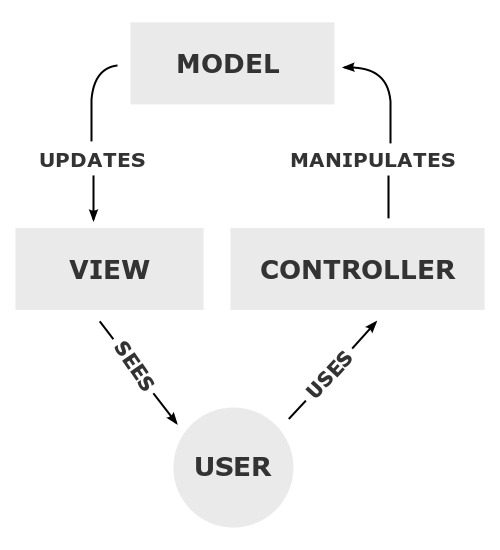
\includegraphics[keepaspectratio, width=0.5\textwidth]{mvc}
  \caption{Interaktion innerhalb des Model-View-Controller Prinzips}
  \label{fig:mvc}
\end{figure}

\noindent
Zusätzlich wurde der Aufbau des Projekts in der \emph{Unified Modelling Language}, kurz \emph{UML}, modelliert.
Dies ermöglicht bereits vor der eigentlichen Implementierung wichtige Begriffe und mögliche Beziehungen festzulegen, und einen Überblick über die benötigten Klassen zu bekommen.

\begin{figure}[h]
  \centering
  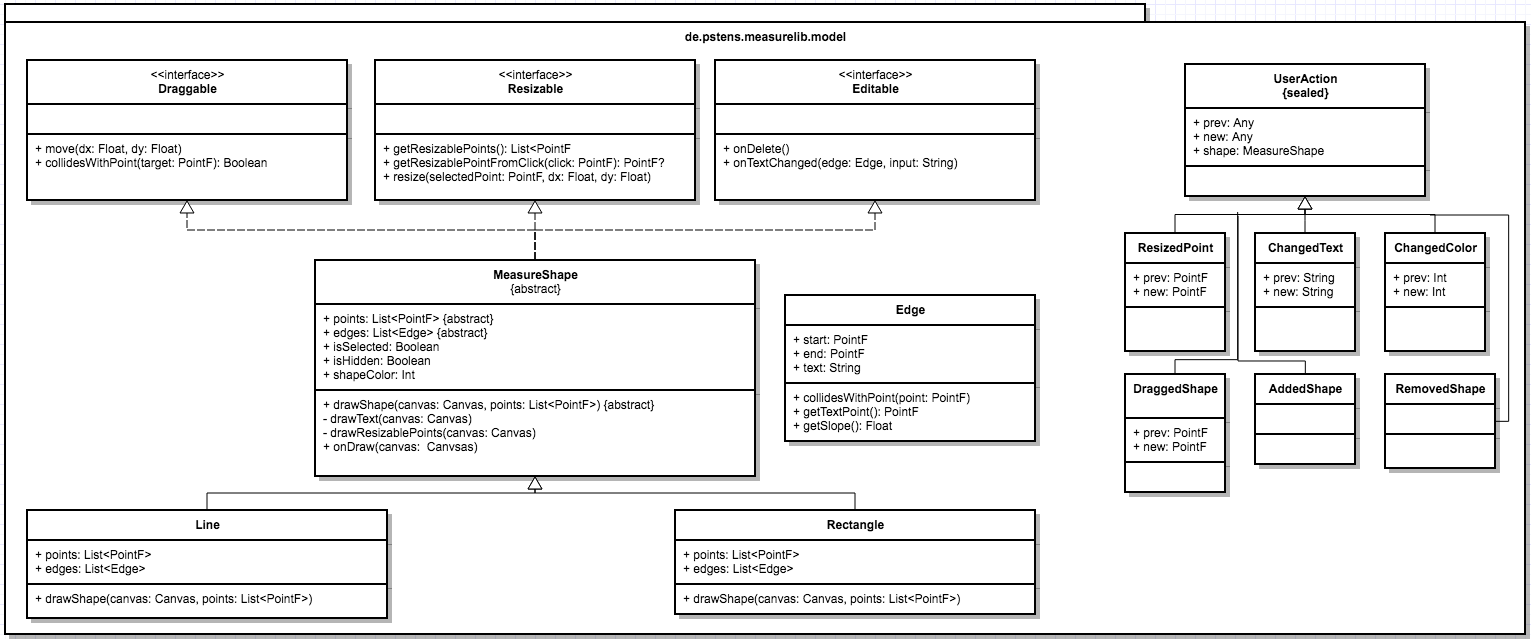
\includegraphics[keepaspectratio, width=\textwidth]{prototype1/model}
  \caption{Datenmodell-Komponente als UML-Diagramm}
  \label{fig:model1}
\end{figure}

\noindent
Die Komponente des \emph{Datenmodells} (siehe \autoref{fig:model1}) sah dabei wie folgt aus (die beiden weiteren Komponenten befinden sich im Anhang):
In \autoref{fig:model1} ist zentral die abstrakte Klasse \emph{MeasureShape} zu erkennen, welche die Oberklasse der beiden Formen \emph{Line} und \emph{Rectangle} darstellt.
\emph{MeasureShape} vererbt die abstrakten Attribute \emph{points} und \emph{edges} an ihre Unterklassen, die diese Attribute in überschreiben müssen.
Außerdem muss die öffentliche Methode \emph{drawShape(...)} von beiden Unterklassen implementiert werden.
Dies sorgt dafür, dass jede Unterklasse selber dafür ``verantwortlich'' ist, wie und wohin ihre Form gezeichnet wird.
\emph{MeasureShape} selber implementiert die drei verschiedene \emph{Interfaces} \emph{Draggable, Resizable und Editable}, welche Schnittstellen zum Verschieben, Vergrößern und Editieren von Formen bereit stellen. \\
\todo{hier nur MeasureShape zeigen und Rest in Anhang}

\noindent
Eine weitere Klasse im \emph{Datenmodell} ist \emph{UserAction}.
Diese ist eine versiegelte (\emph{sealed}) Oberklasse, welche die verschiedenen Benutzeraktionen darstellt.
Versiegelt bedeutet in diesem Kontext, dass nur Klassen, welche im \emph{Scope} der Oberklasse liegen, von dieser erben können.
Folgende sechs Benutzeraktionen können in der Implementierung des ersten Prototyps über die Undo/Redo-Funktion rückgängig gemacht oder wiederhergestellt werden:

\begin{itemize}
  \item Verschieben von Formen (\emph{DraggedShape})
  \item Hinzufügen von Formen (\emph{AddedShape})
  \item Löschen von Formen (\emph{RemovedShape})
  \item Vergrößern bzw. verkleinern von Formen (\emph{ResizedPoint})
  \item Ändern des Textes (\emph{ChangedText})
  \item Ändern der Farbe (\emph{ChangedColor})
\end{itemize}

\noindent
Funktional beschränkt sich die Implementierung des ersten Prototyps zunächst auf das Zeichnen von einfachen Linien und Vierecken, sowie das anschließende Beschriften dieser, um Messwerte einzutragen.
Zum schnellen und präzisen Zeichnen der Formen wird eine Zoom-Linse (siehe \autoref{fig:draw1}), wie sie in allen drei Apps aus \autoref{chap:eval} umgesetzt wurde, verwendet.
Der Prototyp verfügt über zwei verschiedene Modi, den Zeichen- und Text-Modus, zwischen denen mit Hilfe des \emph{Floating Action Buttons} im unteren rechten Bildschirmbereich umgeschaltet werden kann (siehe \autoref{fig:all1}).
Zudem kann der Benutzer über einen weiteren \emph{Floating Action Button} im unteren linken Bildschirmbereich jederzeit ein neues Bild aufnehmen, oder ein bereits vorhandenen in die App importieren. \\

Undo- sowie Redo-Funktion befinden auf dedizierten \emph{Buttons} in der Menüleiste der App (siehe \autoref{fig:all1}).
Hier gibt es außerdem jeweils einen Button, um ausgewählte Formen zu löschen, die Zeichenfarbe zu ändern, oder eine andere Form zum Zeichnen auszuwählen. \\

\begin{figure}[h]
  \begin{subfigure}[t]{0.4\textwidth}
    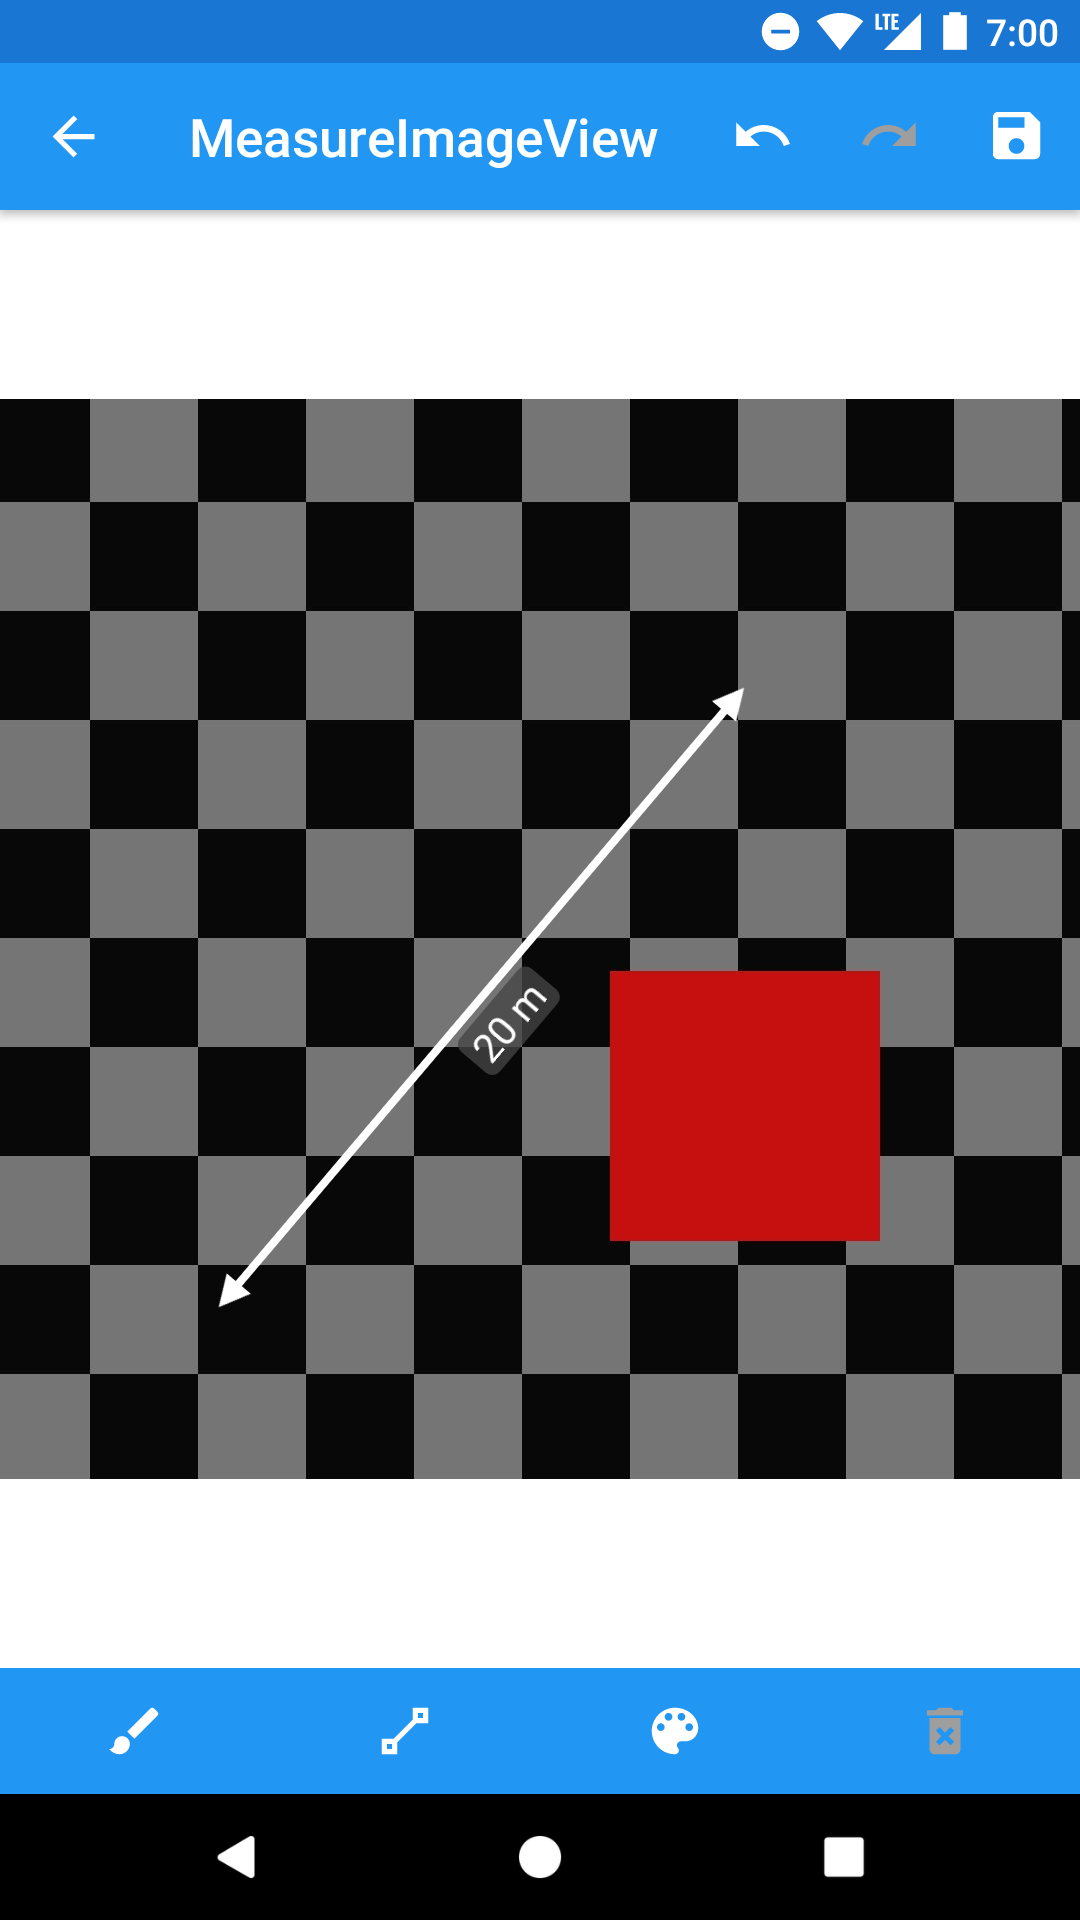
\includegraphics[keepaspectratio, width=\textwidth]{prototype1/all}
    \caption{Erster Prototyp mit bereits eingezeichneter Linie}
    \label{fig:all1}
  \end{subfigure}
  \begin{subfigure}[t]{0.4\textwidth}
    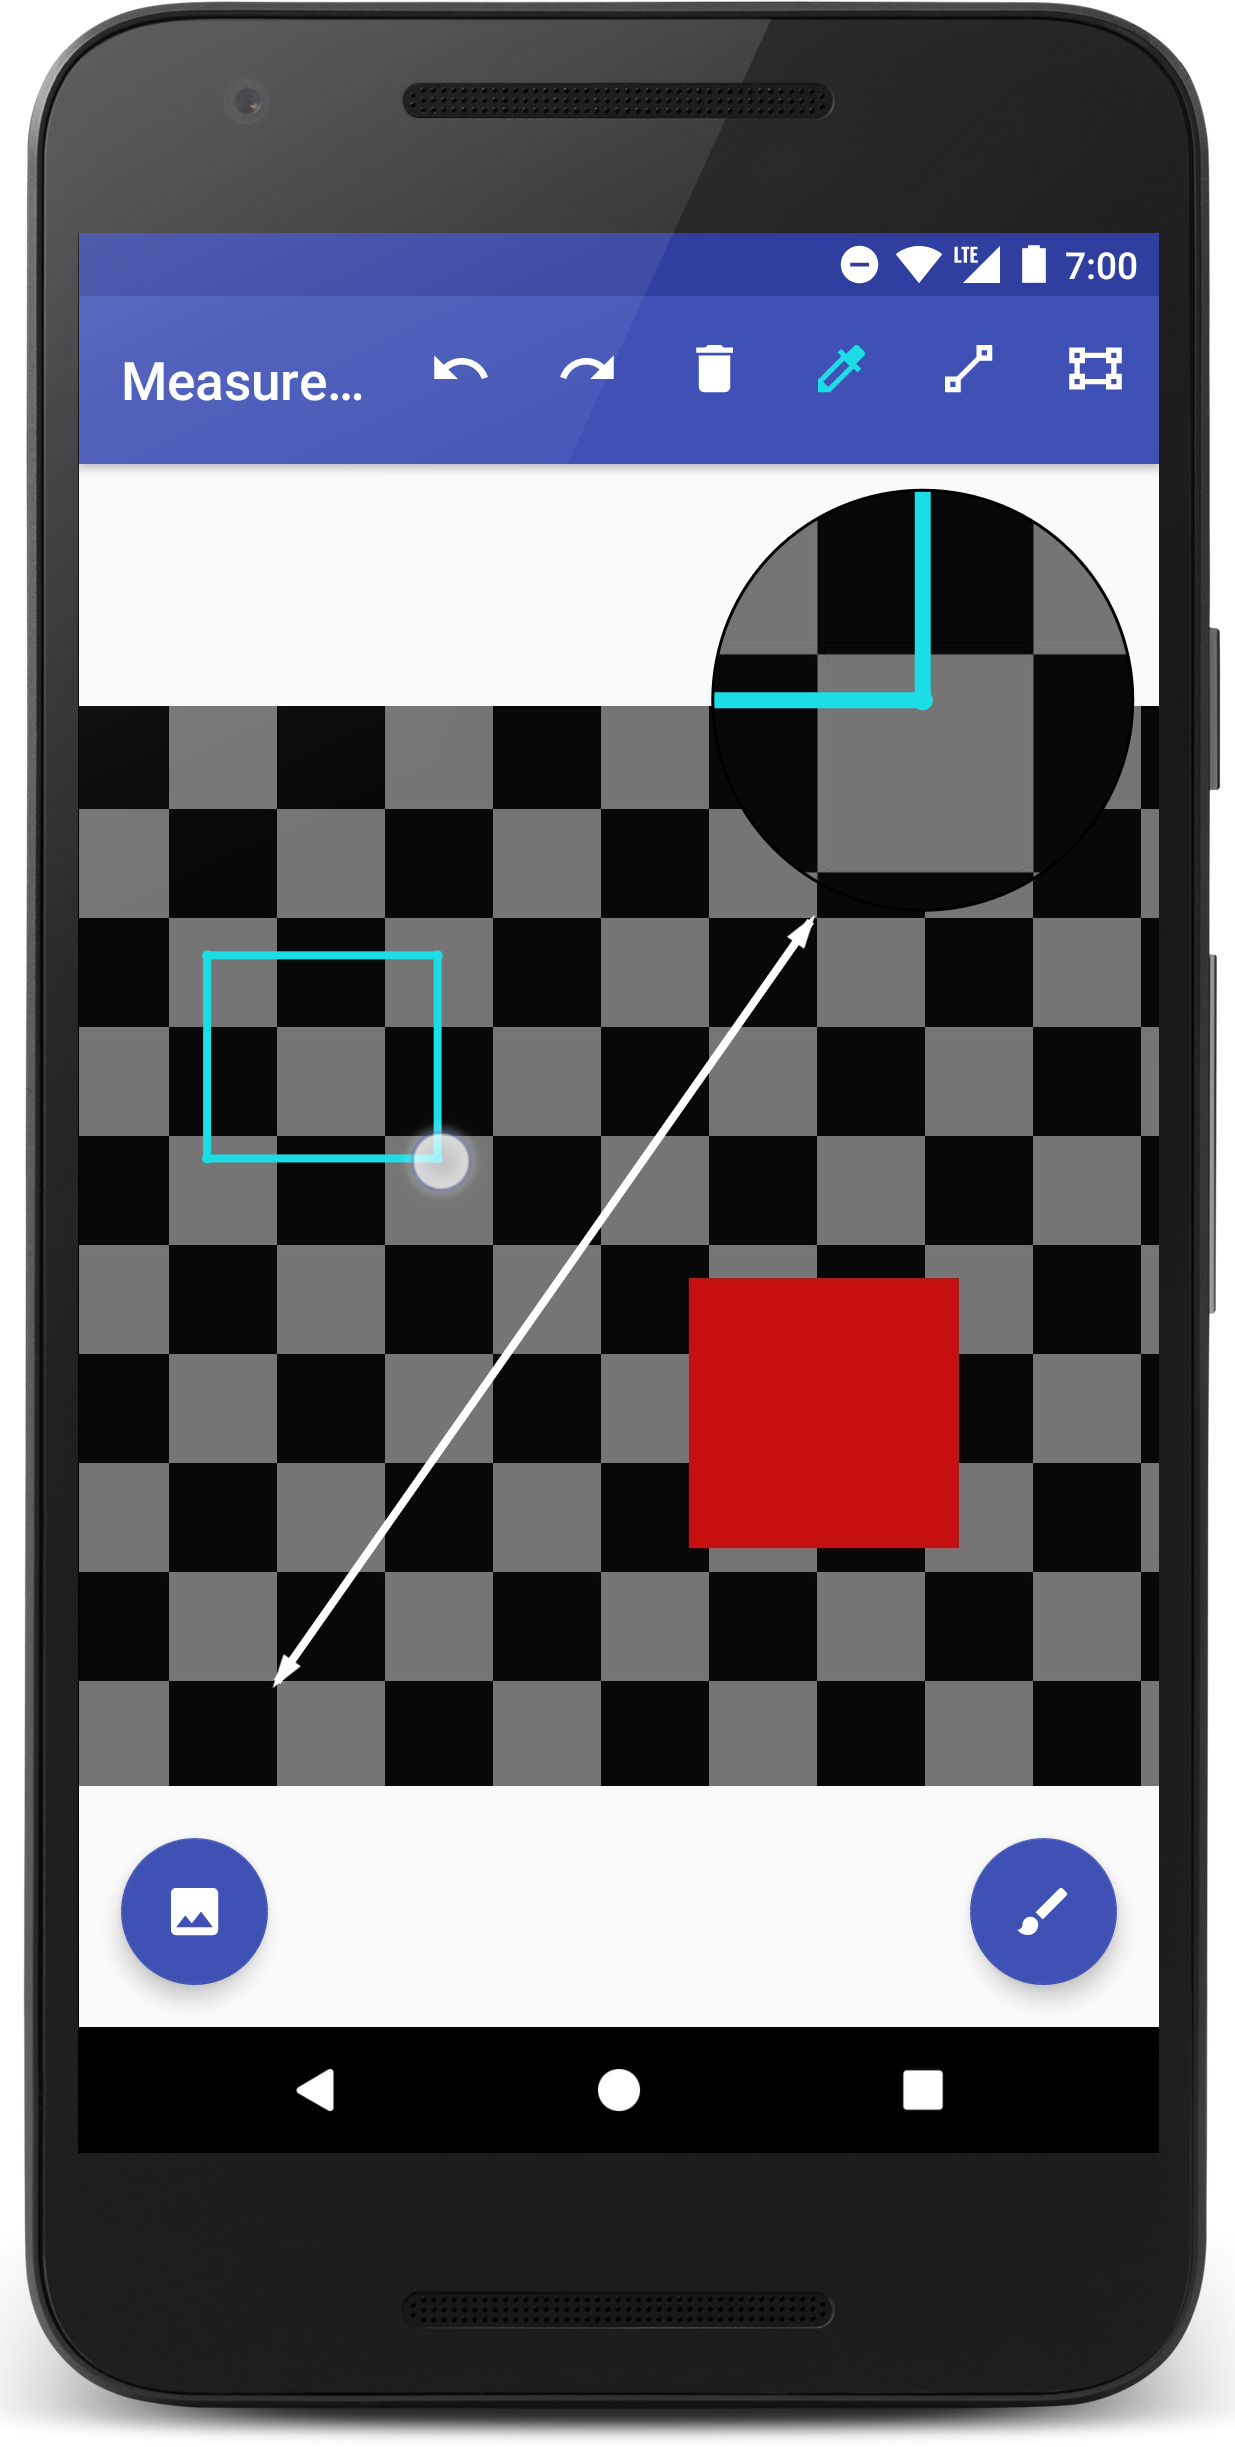
\includegraphics[keepaspectratio, width=\textwidth]{prototype1/drawing}
    \caption{Zoom-Linse beim Zeichnen einen Vierecks}
    \label{fig:draw1}
  \end{subfigure}
  \centering
  \caption{Erster Prototyp bei eingezeichneter Linie und beim Zeichnen eines Vierecks}
\end{figure}

\noindent
Beim Auswählen des Farb-Icons in der Menüleiste öffnet sich ein modaler Dialog, der es dem Benutzer ermöglicht, die gewünschte Farbe auszuwählen (siehe \autoref{fig:color1}).
Diese Farbe wird als Standardfarbe für alle neuen Formen genutzt.
Falls vor dem Öffnen des Dialogs eine Form markiert wurde, wird diese ebenfalls mit der ausgewählten Farbe eingefärbt. \\

\begin{wrapfigure}{R}{0.5\textwidth}
  \centering
  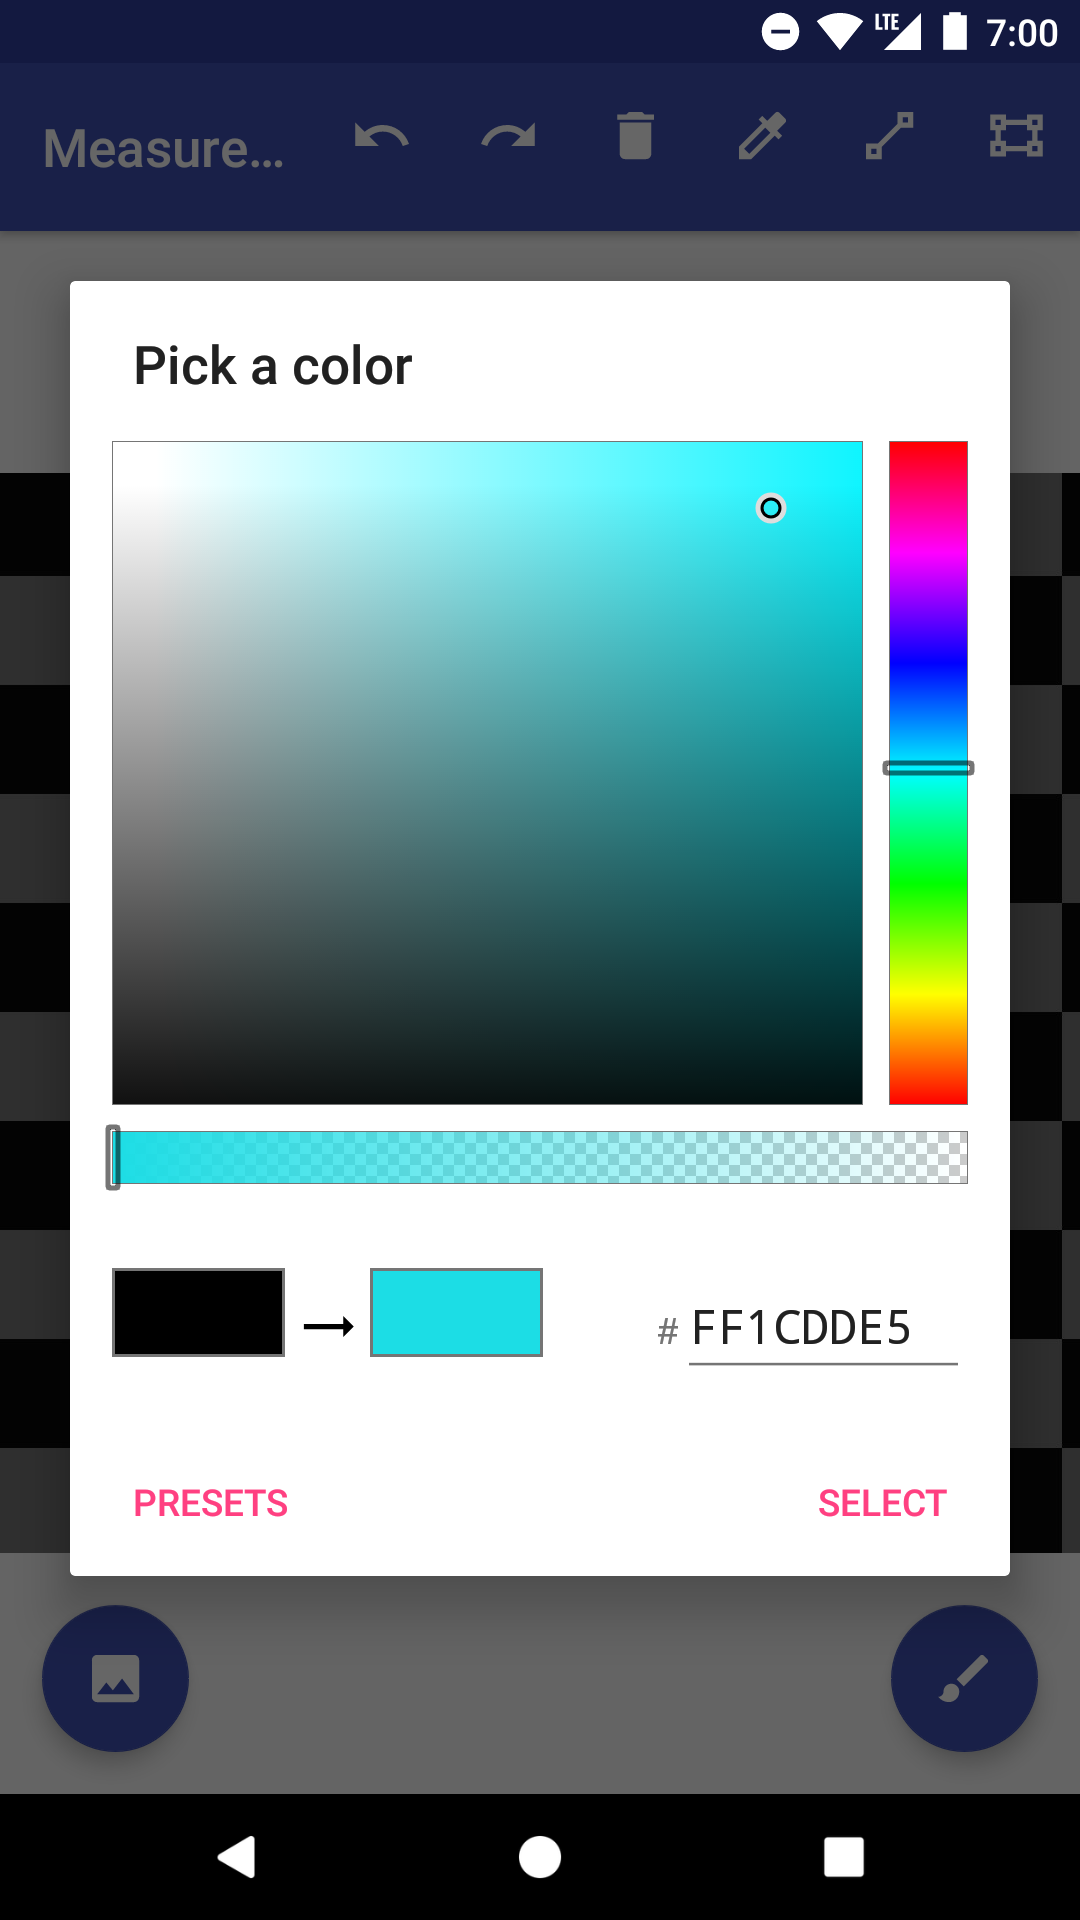
\includegraphics[keepaspectratio, width=0.4\textwidth]{prototype1/color}
  \caption{Geöffneter Farbauswahl-Dialog}
  \label{fig:color1}
\end{wrapfigure}

Graue Indikatoren an den Eckpunkten der aktuell ausgewählte Form sollen dem Nutzer verdeutlichen, dass dieser mit Hilfe der Indikatoren die Form in ihrer Größe und Position bearbeiten kann.
Um Formen zu beschriften bietet sich dem Benutzer im Text-Modus die Möglichkeit, Kanten mittels eines Eingabe-Dialogs zu annotieren (siehe \autoref{fig:labeling1}).
Hierzu öffnet sich beim langen Klick auf die Kante einer Form im Text-Modus ein modaler Dialog, welcher die Messwerte des Nutzers entgegennimmt.
Eingetragene Messwerte werden anschließend neben der zuvor ausgewählten Kante im Bild dargestellt (siehe \autoref{fig:label1}). 
\todo{neues Bild wo Messwert besser sichtbar}

\begin{figure}[h]
  \begin{subfigure}[t]{0.4\textwidth}
    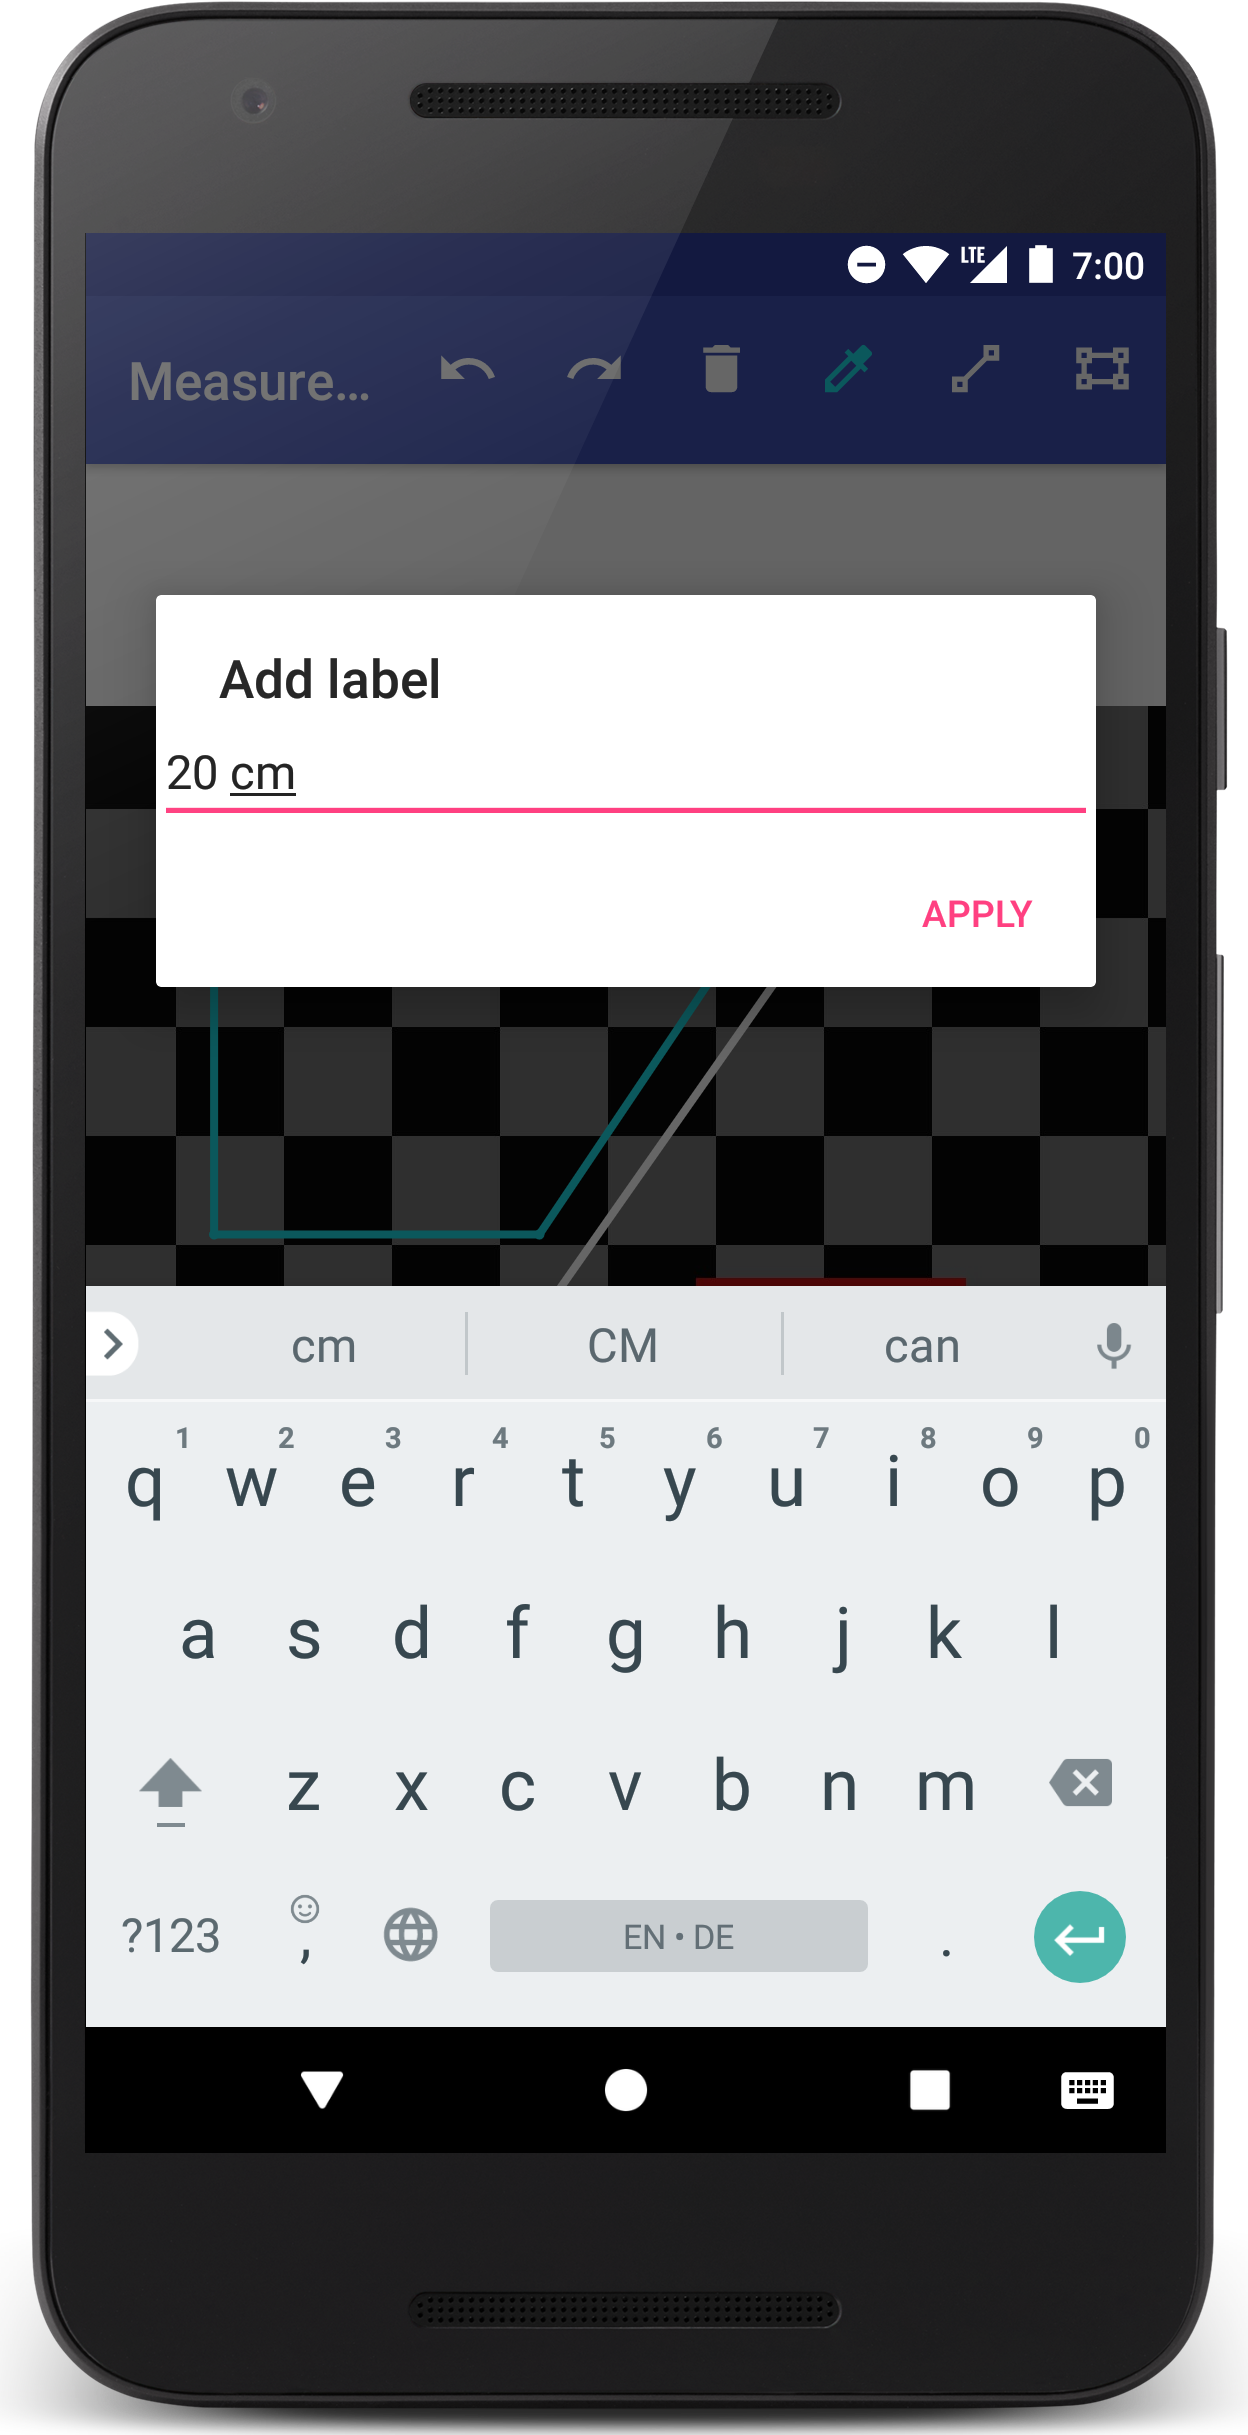
\includegraphics[keepaspectratio, width=\textwidth]{prototype1/labeling}
    \caption{Dialog zum Eintragen von Messwerten}
    \label{fig:labeling1}
  \end{subfigure}
  \begin{subfigure}[t]{0.4\textwidth}
    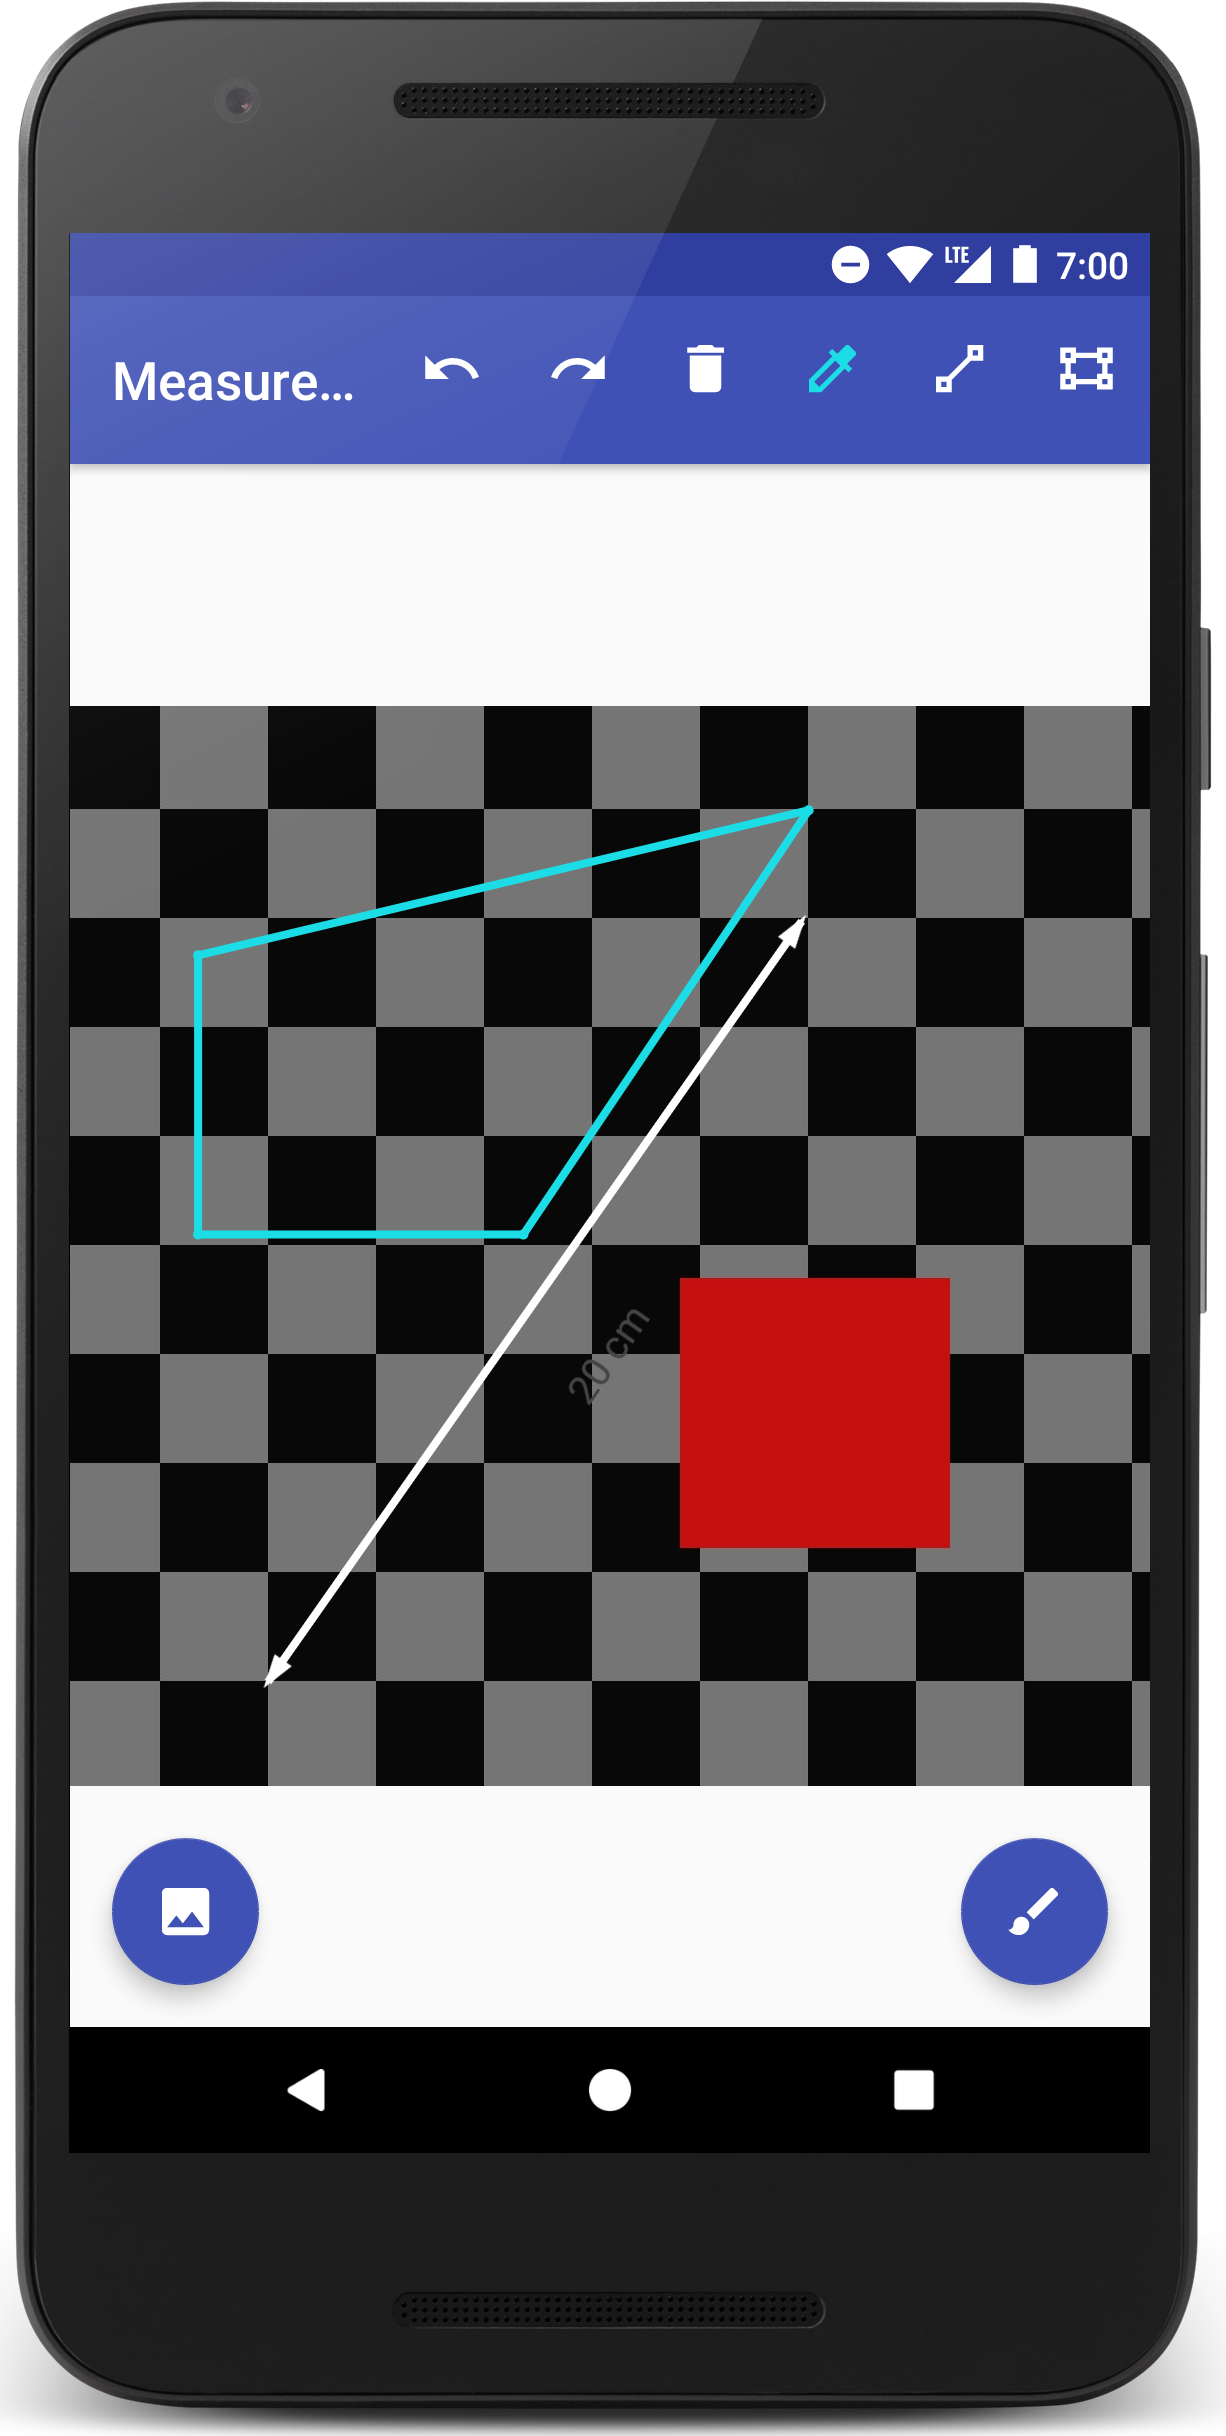
\includegraphics[keepaspectratio, width=\textwidth]{prototype1/label}
    \caption{Linie mit eingetragenem Messwert}
    \label{fig:label1}
  \end{subfigure}
  \centering
  \caption{Eintragen und Anzeigen von Messwerten im ersten Prototyp}
\end{figure}

\section{Test}\label{sec:test1}
Nachdem die App zwei Tage in den Arbeitsalltag der beiden Geschäftsführer der Fa. VERO integriert und währenddessen getestet wurde, gab es am 18. Dezember Feedback zur Implementierung des ersten Prototyps. \\

Nach Aussage beider Testpersonen, haben die \emph{Floating Action Buttons} sich bei der Benutzung der App als großes Hindernis herausgestellt.
So sei nicht intuitiv klar, dass die App über zwei verschiedene Modi, nämlich den Zeichen- und Text-Modus, verfügt.
Zudem sei unklar, dass man über einen Klick auf den rechten \emph{Floating Action Button} zwischen den beiden Modi hin und her wechseln kann. \\

Ein weiteres Problem ergab sich laut Testpersonen X \todo{Wie hier differenzieren?} bei der Benutzung der App auf seinem Tablet.
So seien sämtliche Texte nur schwer lesbar, und diverse Punkte zum Verändern der Formen zu klein, sodass sie nur mühsam und mit viel Konzentration mit dem Finger zu treffen seien. \\

Ein weiteres Problem, was beide Testpersonen schilderten, war die schlechte Lesbarkeit von eingetragenen Messwerten auf Bildern, die in dunkleren Lichtverhältnissen aufgenommen wurden.
Hier setze sich die Textfarbe zu schlecht vom Hintergrund ab. \\

Des Weiteren kam von beiden Testpersonen der Wunsch nach der Möglichkeit, Formen mit bereits vorhandenen Gerüsttypen wie zum Beispiel ``Hängegerüst'' oder ``Standgerüst'' zu verbinden, und in den Meta-Daten des Bildes zu speichern. \\

Außerdem wurde von beiden Testpersonen mehrfach angemerkt, dass es wünschenswert wäre, Bilder vor dem Bearbeiten über eine weitere Oberfläche zunächst zurecht zu schneiden und eventuell drehen zu können.
Dies sei eine essentielle Funktion, da es auf der Baustelle oftmals dazu komme, dass aufgenommene Bilder nicht nur das gewünschte Gerüst, sondern noch andere Objekte, die nicht relevant für das Bild seien, beinhalten. \\

Die Ursachen und mögliche Lösungsideen dieser Probleme sollen im nächsten Abschnitt in einer weiteren Iteration des ``Human-Centered Design Process'' ausgewertet und mit Hilfe eines zweiten Prototyps versucht gelöst zu werden.
